\chapter{Zeitreisen\label{chapter:thema}}
\lhead{Zeitreisen}
\begin{refsection}
\chapterauthor{Sascha Jecklin und Jonas Gründler}

\section{Einleitung}

Das Thema Zeitreisen fasziniert den Menschen schon seit er sich der Zeit bewusst ist. Früh schon entstanden Träume den Verlauf der Zeit manipulieren zu können. Erste schriftliche und bildliche Belege dafür gab es bereits in der Hinduistischen Mythologie und in der Buddhistischen Religion. Auch in der modernen Literatur und in der Filmindustrie sind Zeitreisen ein beliebtes Thema. Klassische Beispiele daf\"ur sind: 

\begin{itemize}
    \item Time Machine, H.G.Wells, 1895 
    \item Das Ende der Ewigkeit, Isaac Asimov, 1955
    \item Back to the Future, 1985-1990
    \item Star Trek
    \item Doctor Who
    \item Interstellar
    \item \ldots
\end{itemize}

\section{Was ist eine Zeitreise}

Eine Zeitreise beschreibt eine Bewegung durch die Zeit, abweichend von der eines Bezugssystems. Man unterscheidet dabei von Reisen in die Vergangenheit oder in die Zukunft. Gerade ersteres wirft schwerwiegende Fragen auf. Was geschieht z.B. wenn der Lauf der Dinge wie sie bis anhin bekannt waren geändert wird? Wenn der Reisende in der Vergangenheit auf sich selber trifft, oder noch absurder gar sein altes ``Ich`` ermordet? 
Mathematisch gesehen wird eine Reise in die Vergangenheit ebenfalls ein wenig anspruchsvoller. Hier beschränken wir uns daher auf Reisen in die Zukunft. 

Natürlich könnte man später argumentieren, dass sich bei gleichbleibender Theorie die Bezugssysteme vertauschen lassen. So könnte man ein Objekt seiner Wahl reissen lassen und sich selber als Bezugssystem sehen. Dies entspricht aber nicht einer Reise in die Vergangenheit sondern lediglich ``weniger schnellem altern``. Das zeitreisende  Objekt könnte trotz Zeit\"anderung immer nur älter sein als zu Beginn der Betrachtung. Obwohl der Beobachter in seinem Bezugssystem einiges schneller gealtert wäre.

Es stellt sich nun die Frage, wie wir mathematisch gesehen eine Zeitreise definieren. Im Abschnitt XXXXXX führten wir den Begriff der Eigenzeit ein. Sie beschreibt die Zeit, welche im Bezugssystem des Reisenden aus der Sicht eines Beobachters vergeht.

Nun müssen wir noch ausformulieren wie wir die Abweichungen von der Eigenzeit erreichen wollen. Die sogenannte Zeitdilatation wie es in der Physik heisst erreicht man entweder durch Geschwindigkeit oder Gravitation. Geschwindigkeit setzt eine zuvorkommende Beschleunigung voraus. Wir wissen bereits, dass Beschleunigung und Gravitation einhergehen. Daher kommt es nicht all zu \"uberaschend, dass wenn das Eine auch das Andere einen Einfluss haben muss.

Wie wir sehen werden bringen schon kleinste \"Anderungen eine Zeitänderung mit sich. Da die praktische Anwendung in diesem Kapitel im Fordergrund steht, interessieren uns in erster Linie natürlich signifikante Unterschiede. Erst doppelt oder sogar zehnfach- schneller vergehenden Eigenzeiten w\"urden uns Effekte best\"atigen, welche man sie uns in Science Fiction Filmen und Romanen verspricht.

\subsection{Geschwindigkeit}

Eine M\"oglichkeit diesen eine Zeitdillatation zu erreichen ist durch hohe Geschwindigkeit. Wenn sich eine Person relativ zu einem Bezugssystem schnell bewegt, vergeht f\"ur diese Person die Zeit im Vergleich zum Bezugssystem langsamer. Die Ver\"anderung wird durch den Lorentzfaktor beschrieben, welcher sich aus der Lorentztransformation herleiten l\"asst. Er beschreibt das Verh\"altnis zwischen der Eigenzeit und der Zeit des Bezugssystems.

\begin{equation}
    \gamma=\frac{1}{\sqrt{1-\frac{v^2}{c^2}}} 
\end{equation}



Die Eigenzeit ist also:

\begin{equation}
    \tau
    =
    \int_{}^{}\frac{1}{\gamma}dt=\int_{}^{}\sqrt{1-\frac{v^2}{c^2}}dt
    =
    \frac{1}{c}\int_{}^{}\sqrt{g_{\mu\nu}\dot{x}^{\mu}(s)\dot{x}^{\nu}(s)}ds
\end{equation}

Diese Formel ist in dieser Form noch nicht sehr Anschaulich. Sie Beschreibt nur, dass eine Metrik mit den jeweiligen Basisvektoren "multipliziert" werden muss(Einsteinsche Summenkonvention). Von dem Ganzen die Wurzel ziehen und dann noch integrieren.
Durch das Einsetzen der Minkowski-Metrik, welche Raum und Zeit miteinander verbindet, und der Basisvektoren $t, x, y, z$ l\"asst sich eine Verst\"andliche Form herleiten. 

Minowski-Metrik:

\begin{equation}
    g_{\mu\nu}=
    \begin{pmatrix}
        -1 & 0 & 0 & 0 \\
        0 & 1 & 0 & 0 \\
        0 & 0 & 1 & 0 \\
        0 & 0 & 0 & 1
    \end{pmatrix}
\end{equation}

Standard Vierervektor:

\begin{list}{}{}
    \item \(x^{0}=ct\)
    \item \(x^{1}=x\)
    \item \(x^{2}=y\)
    \item \(x^{3}=z\)
\end{list}

Ein wenig Umstellen und vereinfachen und man kommt auf diese Form:

\begin{equation}
    \tau
    =
    \frac{1}{c}\int_{}^{}\sqrt{-(-c^2\dot{t}(s)^{2}+\dot{x}(s)^{2}+\dot{y}(s)^{2}+\dot{z}(s)^{2})}ds
\end{equation}

Je nachdem wie die Bewegung gew\"ahlt wird, fallen einer oder mehrere der Basisvektoren  $x, y, z$ weg.

Hier ein Beispiel bei welchem nur eine Geschwindigkeit in x-Richtung vorhanden ist (c=Lichtgeschwindigkeit, u beschreibt den Bruchteil):

\begin{list}{}{}
    \item $t(s)=1s, \dot{t}(s)=1$
    \item $x(s)=u*c*s, \dot{x}(s)=u*c$
    \item $y(s)=0, \dot{y}(s)=0$
    \item $z(s)=0, \dot{z}(s)=0$
\end{list}

\begin{align*}
    \tau
    &=
    \frac{1}{c}\int_{}^{}\sqrt{-(-c^2\dot{t}(s)^2+\dot{x}(s)^2)}ds 
    =
    \frac{1}{c}\int_{}^{}\sqrt{-(-c^2*1+(u*c)^{2}}ds\\
    &=
    \frac{s*\sqrt{c^2+(u*c)^{2}}}{c} 
    =
    s*\sqrt{1-\frac{u^2*c^2}{c^2}}
\end{align*}

Welches die einfachste Form einer Zeitdilatation darstellt.\\
\\
Hier ein Zahlenbeispiel bei welchem zuf\"allige Werte gew\"ahlt wurden:
$s=5000, u=0.2$ 

\begin{list}{}{}
    \item $t(s)=1s, \dot{t}(s)=1$
    \item $x(s)=0.2cs, \dot{x}(s)=0.2c$
    \item $y(s)=0, \dot{y}(s)=0$
    \item $z(s)=0, \dot{z}(s)=0$
\end{list}

\begin{align*}
    \tau
    &=
    \frac{1}{c}\int_{s_{a}}^{s_{b}}\sqrt{-(-c^2\dot{t}(s)^2+\dot{x}(s)^2)}ds
    &=
    \frac{1}{c}\int_{0}^{5000}\sqrt{-(-c^2+((0.2c)^2))}ds\\
    &=
    5000*\sqrt{1-\frac{u^2*c^2}{c^2}} = 4898.98
\end{align*}

Dieses Beispiel zeigt auch, dass eine relevante Zeitverlangsamung erst bei sehr hohen Geschwindigkeiten erreicht wird

\begin{figure}
    \centering
    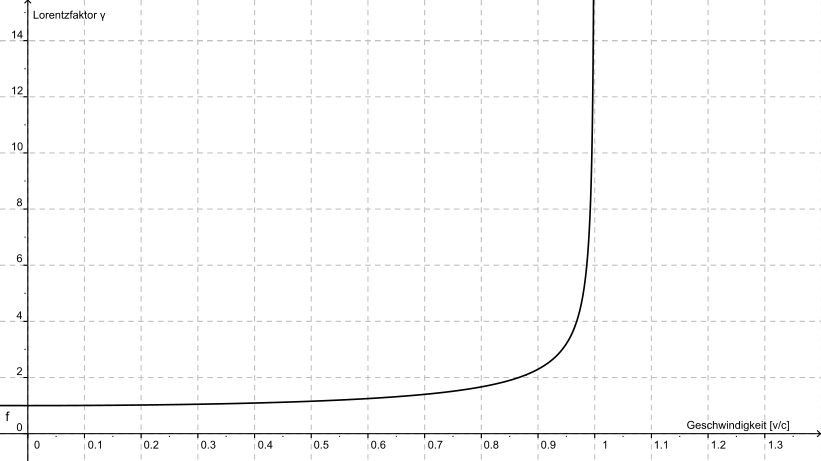
\includegraphics[width=\hsize]{zeitreisen/Lorentzfaktor.jpg}
    \caption{Ver\"anderung des Lorentzfaktor in Abh\"angigkeit der Geschwindigkeit%
        \label{skript:geodaten:fig:transport}}
\end{figure}

\subsection{Gravitation}

	In diesem Kapitel beschäftigen wir uns mit dem Einfluss der Gravitation auf die Zeit. Gravitation muss durch eine Krümmung des Raumes beschrieben werden. Erkennen lässt sich die Gravitation z.B. an der Anziehungskraft der Erde. Alles wird mit $g=9.81\frac{m}{s^2}$ in Richtung Erdmittelpunkt beschleunigt. $F=\frac{KMm}{r^2}$
	Die Beschleunigung ist also unabhängig von der Masse.
	Ein beschleunigtes Koordinatensystem kann zwar durch eine Koordinatentransformation erreicht werden, doch diese ist keine Lorentztransformation und lässt sich nicht durch die die Minkowski-metrik darstellen.\\ Der Ansatz $ -c^2dt^2 + dx^2 + dy^2 + dz^2$ genügt nicht mehr. Wir müssen also Metriken und Transformationen zulassen, welche von der Minkowski-Metrik und der Standarttransformation abweichen.\\
	Eine Metrik, welche wir für unsere Zwecke benützen können, ist die Schwarzschild-Metrik. Sie berücksichtigt die Gravitation, durch eine Krümmung des Raumes dargestellt, und beschreibt so Gravitationsfelder in der nähe von massereichen Objekten. Diese Lösung wurde von Karl Schwarzschild nur wenige Monate nach der Präsentierung der Einsteinschen Feldgleichungen gefunden. Aus ihr lassen sich Bewegungsgleichungen von Körpern in einem Gravitationstrichter herleiten.\\\\
	Die Schwarzschildmetrik in Vektordarstellung:



	\begin{equation}
		g_{\mu\nu}=
		\begin{pmatrix}
		-\biggl(-1-\frac{r_{g}}{r}\biggr) & 0 & 0 & 0 \\
		0 & \frac{1}{\displaystyle1-\frac{r_{g}}{r}} & 0 & 0 \\
		0 & 0 & r^{2} & 0 \\
		0 & 0 & 0 & r^{2}\sin^{2}(\vartheta)
		\end{pmatrix}
	\end{equation}

	Der Vierervektor in Kugelkoordinaten:

	\begin{list}{}{}
		\item \(x^{0}=ct\)
		\item \(x^{1}=r\)
		\item \(x^{2}=\vartheta\)
		\item \(x^{3}=\varphi\)
	\end{list}

	Daraus lässt sich die Längenmessung zusammenstellen. Auf die Herleitung der Schwarzsdchild-Metrik verzichten wir an dieser Stelle.

	\begin{equation}
	ds^2
	=
	-\biggl(1-\frac{r_g}r\biggr)c^2dt^2
	+
	\frac{1}{\displaystyle 1-\frac{r_g}r}\,dr^2 
	+
	r^2d\vartheta^2 
	+ 
	r^2\sin^2(\vartheta)d\varphi
	\end{equation}

	$r_g$ beschreibt den Gravitationsradius(Ereignishorizont) des betrachteten Körpers.

	\subsubsection{Bedeutung von $R_{g}$ und Ereignishorizonte}


	Der Ereignishorizont beschreibt in der allgemeinen Relativitätstheorie eine Grenzfläche dar. Er beschreibt die Entfernung ab welcher das Licht nicht mehr aus der Gravitationstrichter entkommen kann. Teilchen die den Ereignishorizont passiert haben, können diesen nicht mehr verlassen. Alles ausserhalb dieses Radius hätte die Möglichkeit zu entkommen, die frage ist nur wie viel Energie benötigt wird. Da Licht nicht mehr entkommen kann nennt man diese Körper auch schwarze Löcher.\\
	Der Gravitationsradius lässt sich mit 

	\begin{equation}
	r_{g}= \frac{2MG}{c^2}
	\end{equation}

	berechnen.
	Der Gravitationsradius der Erde beträgt etwa 8.8mm. Wenn wir die Erde also unter  diese 8.8mm komprimieren, würde sie sich in ein schwarzes Loch verwandeln. Ihre Dichte wäre dann so gross, dass nichts mehr der Anziehung widerstehen kann.
	%do vlt no chli was... weiss aber nonig genau was
	
	\subsection{Realisierbarkeit}
	
	%probleme mit Reiseweg, und nur kleine Zeiteinssparung bei 20%c
	%energie
	
	\subsubsection{Lasersegel}
	%Bsp Laser mit lichtsegel...
	
	\section{Umkreisung}
	
	
	%am Sagitarrius A* angekommen: -Gesteuerte Bahn
	%							   -lösung mit geodäten
	
	\subsubsection{gesteuerte Bahn}
	
 	%kurze erklärung, probleme energie für gesteuerte bahn, ...
	
	\subsubsection{Geodätenlösung}
	
	%"herleitung" geodätegleichung
	%Christoffelsymbole berechnung und aufstellung
	%einsetzen und erstellung der Diffgleichungen für simulation
	
	\subsection{Simulation}
	
	%Erklärung sourcecode
	
	\subsection{fazit}
	
	%üseri erkenntnis us de arbet
	
	


	\printbibliography[heading=subbibliography]
	\end{refsection}

